\section{Electronical formulas}
	

\begin{figure}[!h]
\centering
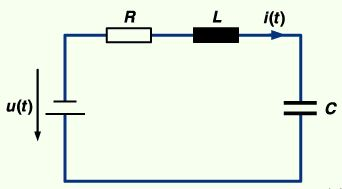
\includegraphics[width=0.7\linewidth]{images_Form/RLC}
\caption{RLC circuit}
\label{fig:RLC}
\end{figure}

\mysubsection{Resistor}
\begin{align}
	u_R(t) = R \cdot i_R(t)
\end{align}
U: voltage [Volt V] \\
R: restistance [Ohm $\varOmega = \frac{V}{A}$] \\
I: current [Ampere A]

\mysubsection{Capacitor/Condenser}
\begin{align}
	Q &= C \cdot U_C \\
	Q &= \int i_C(t) \\
	i_C(t) &= C \cdot u_C^\prime(t)
\end{align}
Q: electric charge [Coulomb C = As] \\
C: capacity [Farad F = $\frac{C}{V}$]

\mysubsection{Inductor}
\begin{align}
	u_L(t) = L \cdot i_L^\prime(t)
\end{align}
L: inductance [Henry H = $\frac{Vs}{A}$]

\newpage
\section{Mechanical formulas}

\mysubsection{Newton's Second Law}
\begin{align}
F = m \cdot a = m \cdot x^{\prime\prime}(t)
\end{align}
m: mass [gramm g] \\
a: acceleration [$\frac{m}{s^2}$]
x: length [meter m]
\mysubsection{Gravitational force}
\begin{align}
F_G = m \cdot g 
\end{align}
g: gravitational acc. [$\frac{m}{s^2}$] (Germany 9.81 $\frac{m}{s^2}$)

\mysubsection{Spring force}
\begin{align}
F_S = k \cdot x
\end{align}
k: spring constant [$\frac{kg}{s^2}$]\\

\mysubsection{Friction force}
\begin{align}
F_F = r \cdot v = r \cdot x^\prime(t)
\end{align}
r: friction constant \\
v: velocity [$\frac{m}{s}$]

\mysubsection{Rotational force}
\begin{align}
F_R = F_G \cdot \sin\rho
\end{align}
$\rho$: angle of displacement

\mysubsection{Torque}
\begin{align}
M = F \cdot r
\end{align}
r: radius

\mysubsection{Rotational movement}
\begin{align}
M = J \cdot \rho^{\prime\prime}
\end{align}
J: moment of inertia \\
$\rho^{\prime\prime}$: angular velocity

